\documentclass[9pt]{pnas-new}
% Use the lineno option to display guide line numbers if required.
% Note that the use of elements such as single-column equations
% may affect the guide line number alignment. 

\RequirePackage[slovene,english]{babel} % when writing in slovene
%\RequirePackage[slovene,english]{babel} % when writing in english

\templatetype{pnasresearcharticle} % Choose template 
% {pnasresearcharticle} = Template for a two-column research article
% {pnasmathematics} = Template for a one-column mathematics article
% {pnasinvited} = Template for a PNAS invited submission

\selectlanguage{english}
% \etal{in sod.} % comment out when writing in english
% \renewcommand{\Authands}{ in } % comment out when writing in english
% \renewcommand{\Authand}{ in } % comment out when writing in english

\newcommand{\set}[1]{\ensuremath{\mathbf{#1}}}
\renewcommand{\vec}[1]{\ensuremath{\mathbf{#1}}}
\newcommand{\uvec}[1]{\ensuremath{\hat{\vec{#1}}}}
\newcommand{\const}[1]{{\ensuremath{\kappa_\mathrm{#1}}}} 

\newcommand{\num}[1]{#1}

\graphicspath{{./fig/}}

\title{Sheepdog-Driven Algorithm for Sheep Herd Transport}

% Use letters for affiliations, numbers to show equal authorship (if applicable) and to indicate the corresponding author
\author{Idora Ban}
\author{Simon Hehnen}
\author{Iva Idzojtic}
\author{Lukas Pucher}

\affil{Collective behaviour course research seminar report} 

% Please give the surname of the lead author for the running footer
\leadauthor{Hehnen} 

\selectlanguage{english}

% Please add here a significance statement to explain the relevance of your work
% \significancestatement{Procedural generation of a tropic island and \\coral reef}{In computer graphics there is frequent need for displaying large vistas of natural looking terrain. Designing such terrain by hand is typically time consuming. With procedural generation, on the other hand, larger areas of natural looking terrain can be generated with or without minimal intervention in a relatively short time. In this work we present a process of procedural generation of a tropical island with the associated corral reef. We start by generating a heightmap for the base terrain. The heightmap is then transformed by simulating the processes of hydraulic and thermal erosion to achieve a more natural look of the terrain. As coral reefs often grow around tropical islands, we also simulate their growth as part of the last step. Real-time visualization is enabled during the simulation, so that one can observe the evolution of the terrain. Here we dynamically apply textures to the terrain based on its local characteristics. The result is a natural looking model of the textured tropical island and corral reef.}{Procedural generation | Terrain generation | Thermal and hydraulic erosion | Coral reef | Simulation | GPU}

\selectlanguage{slovene}
\usepackage{verbatim}

\usepackage{graphicx}
\usepackage{subcaption}
\usepackage{float}
% Please include corresponding author, author contribution and author declaration information
%\authorcontributions{Please provide details of author contributions here.}
%\authordeclaration{Please declare any conflict of interest here.}
%\equalauthors{\textsuperscript{1}A.O.(Author One) and A.T. (Author Two) contributed equally to this work (remove if not applicable).}
%\correspondingauthor{\textsuperscript{2}To whom correspondence should be addressed. E-mail: author.two\@email.com}

% Keywords are not mandatory, but authors are strongly encouraged to provide them. If provided, please include two to five keywords, separated by the pipe symbol, e.g:
\keywords{Sheepdog-Driven algorithm | Swarm systems | Controlling agent} 

\begin{abstract}
%The project explores the sheepdog-driven algorithm for sheep herd transport, demonstrating how a single agent can control and guide a swarm from one location to another through simple local interactions. The objective is to replicate the algorithm and evaluate its effectiveness in simulating dynamic control, where the sheepdog influences the herd's movement using basic rules. The backward semi-circle reciprocation algorithm will be implemented, incorporating behaviors observed in real sheepdogs, such as circular path movement and decision-making based on the sheep's positions. The effectiveness of the algorithm in achieving coordinated herd transport will be assessed under varying conditions, including changes in herd size, obstacle placement, and sheepdog responsiveness. Ultimately, the goal is to enhance the algorithm’s adaptability and explore its broader potential.

This project explores the Sheepdog-Driven Algorithm for Sheep Herd Transport, which demonstrates how a single agent can guide and control a swarm from one location to another using simple local interactions. The goal was to replicate and evaluate the algorithm’s performance in directing a herd with a single controlling agent.
A simulation and 3D visualization were developed to model and analyze the interactions between the sheepdog and the herd. The algorithm effectively demonstrated realistic behaviors, including attraction, repulsion, and visibility-based interactions, showcasing how local rules can influence collective movement. However, challenges in implementation prevented the herd from consistently reaching the target, highlighting areas where further refinement is needed.
\end{abstract}

\dates{\textbf{\today}}
\program{BM-RI}
\vol{2024/25}
\no{CB:G1} % group ID
\fraca{FRIteza/201516.130}

\begin{document}

% Optional adjustment to line up main text (after abstract) of first page with line numbers, when using both lineno and twocolumn options.
% You should only change this length when you've finalised the article contents.
\verticaladjustment{-2pt}

\maketitle
\thispagestyle{firststyle}
\ifthenelse{\boolean{shortarticle}}{\ifthenelse{\boolean{singlecolumn}}{\abscontentformatted}{\abscontent}}{}


\section*{Introduction}

\dropcap{A}nimal behavior-inspired algorithms enable efficient, adaptive solutions to complex problems by mimicking the coordinated actions of animals, swarm behaviours, such as flocking or schooling. This project explores the Sheepdog-Driven Algorithm for Sheep Herd Transport by Liu et al., 2021 \cite{liu2021}, that moves beyond traditional swarm systems, where collective behavior emerges naturally within a group, to address a reverse problem: how a single agent (a "sheepdog") can control and direct a swarm (a "herd of sheep") from one location to another.
 The objective is to replicate and evaluate this sheepdog-inspired approach, focusing on how a single controlling agent can dynamically influence the herd to accomplish transport tasks. The aim is to implement the algorithm from scratch, which allows for a deeper understanding of its mechanics and provides a more flexible, library-free approach to controlling the herd.

%After implementing the base algorithm, our team will experiment with its parameters and performance under different conditions. This will include testing variations like obstacle placement, changes in herd size, or adjustments to sheepdog responsiveness. As we analyze the algorithm’s effectiveness in guiding the sheep herd, we may consider developing new behaviors or optimizations to enhance adaptability, with the potential for further applications in fields like autonomous drone or robot control.





\subsection*{Related Work}

%In recent years, numerous studies have advanced the understanding of collective behavior and herding control among autonomous agents. A foundational contribution by Reynolds (1987) \cite{reynols1987} introduced the "boids" model, which used local rules to simulate natural group dynamics such as flocking and schooling. This work laid the groundwork for many modern algorithms in swarm robotics and serves as an essential reference for simulating decentralized animal behaviors. 
%They suggested that future work could involve adding more realistic individual behaviors, such as hunger or fear, and integrating detailed animations like wing flapping with motion dynamics. These enhancements could make simulations more lifelike and versatile.


%Building on this, Strömbom et al. (2014) \cite{Strmbom2014SolvingTS} addressed the specific "shepherding problem," proposing heuristic methods for guiding groups of autonomous agents using a single "shepherd" agent—a framework that highlights key challenges and strategies relevant to single-agent control in herding tasks. Their approach emphasizes adaptive switching between collecting agents that are dispersed and driving the group when it is cohesive, a behavior closely resembling real-world herding events involving sheep and sheepdogs. Notably, their algorithm also highlights the importance of visual feedback, such as estimating spacing between agents, to maintain group cohesion and movement toward a target.
%This method demonstrates broader applicability, from robot-assisted herding and crowd control to tasks like environmental cleanup, making it a versatile solution for various collective behavior scenarios.


%Furthermore, Bayazit, Lien, and Amato (2002) \cite{bayazit2002} proposed a global roadmap approach for managing group behavior in complex, obstacle-rich environments, underscoring strategies for effective navigation in challenging terrains. They demonstrated how embedding behavior rules into roadmaps and individual agents enables dynamic decision-making based on location and state. This approach mirrors the Sheepdog-Driven Algorithm, where the sheepdog dynamically adjusts its behavior based on the herd’s position and proximity to obstacles. Both frameworks rely on balancing local interactions with global guidance, ensuring that individual agents respond adaptively while maintaining overall group cohesion. The roadmap's ability to represent environmental constraints and influence movement aligns with the algorithm's goal of efficiently directing herds in diverse and complex scenarios.

Recent studies have advanced the understanding of collective behavior and herding control among autonomous agents. Reynolds (1987) \cite{reynols1987} introduced the "boids" model, using local rules to simulate group dynamics like flocking and schooling. This work laid the foundation for modern swarm robotics algorithms and decentralized animal behavior simulations.

Strömbom et al. (2014) \cite{Strmbom2014SolvingTS} addressed the "shepherding problem," proposing methods for guiding groups with a single "shepherd" agent. Their approach emphasizes adaptive switching between collecting dispersed agents and driving cohesive groups, resembling real-world herding. It also highlights the importance of visual feedback, such as agent spacing, to maintain cohesion and target movement. This method applies to robot-assisted herding, crowd control, and environmental cleanup.

Bayazit, Lien, and Amato (2002) \cite{bayazit2002} proposed a global roadmap approach for managing group behavior in complex environments. By embedding behavior rules into roadmaps, agents dynamically make decisions based on location and state. This mirrors the Sheepdog-Driven Algorithm, where the sheepdog adjusts its behavior based on the herd’s position and obstacles, balancing local interactions with global guidance to efficiently direct herds in complex scenarios.

Together, these studies form a comprehensive base for understanding swarm and herding behaviors, which informs the development of adaptive and efficient algorithms, such as the Sheepdog-Driven Algorithm, and supports a comparative analysis of its performance across various environments and control requirements.



\begin{comment}
\begin{algorithm}[H]
\caption{Sheepdog Driven Algorithm \cite{liu2021}}
\label{alg:sheepdog}
\textbf{Input:} $p_1(t), \dots, p_n(t), q(t), \lambda(k)$. \\
\textbf{Output:} $u(k)$.
\begin{algorithmic}[1]
\State Set $\varpi = 0$.
\For{$(i = 1, i \leq N, i = i + 1)$}
    \If{$d(p_i(t), P_d) = 0$}
        \State $\varpi = \varpi + 1$.
    \EndIf
\EndFor
\If{$\varpi < N$}
    \If{$q(k) \in Q_l(k)$ \textbf{and} $L_c(k) > \theta_t$}
        \State $\lambda(k) = 0$.
        \If{$\|q(k) - D_r(k)\| \geq r_a$}
            \State $u(k) = \gamma_a o(q(k) - D_r(k))$.
        \Else
            \State $u(k) = \gamma_b R(\theta_r) o(q(k) - D_r(k))$.
        \EndIf
    \ElsIf{$q(k) \in Q_r(k)$ \textbf{and} $R_c(k) > \theta_t$}
        \State $\lambda(k) = 1$.
        \If{$\|q(k) - D_l(k)\| \geq r_a$}
            \State $u(k) = \gamma_a o(q(k) - D_l(k))$.
        \Else
            \State $u(k) = \gamma_b R(\theta_l) o(q(k) - D_l(k))$.
        \EndIf
    \ElsIf{$\lambda(k) = 1$}
        \If{$\|q(k) - D_l(k)\| \geq r_a$}
            \State $u(k) = \gamma_a o(q(k) - D_l(k))$.
        \Else
            \State $u(k) = \gamma_b R(\theta_l) o(q(k) - D_l(k))$.
        \EndIf
    \Else
        \If{$\|q(k) - D_r(k)\| \geq r_a$}
            \State $u(k) = \gamma_a o(q(k) - D_r(k))$.
        \Else
            \State $u(k) = \gamma_b R(\theta_r) o(q(k) - D_r(k))$.
        \EndIf
    \EndIf
\Else
    \State $u(k) = 0$.
\EndIf
\State \textbf{return} result
\end{algorithmic}
\end{algorithm}
\end{comment}

\section*{Methods}

The practical component of this project is divided into two primary tasks: implementing the simulation algorithm in Python and developing a visualization system in Unity. The methodology section outlines the approach taken to develop these components, along with the processes for testing, refining, and analyzing results.

\subsection*{The Algorithm}
The algorithm defines the sheepdog’s movement as a backward semi-circular trajectory, allowing it to drive the sheep herd from behind \cite{liu2021}. The sheepdog operates within a two-dimensional plane, using an xx-yy coordinate system to track both its own location and that of each sheep. The sheepdog aims to guide the herd toward a designated target area by pushing them forward in a controlled manner.

Key aspects of the algorithm include the sheepdog's field of view, which restricts its awareness to only those sheep within its line of sight. Consequently, the sheepdog's response is dynamically adjusted based on the position and behavior of visible sheep, meaning it does not always have complete information about the entire herd.

\begin{comment}   
\begin{figure}[H]
    \centering
    \begin{subfigure}{0.48\textwidth}
        \centering
        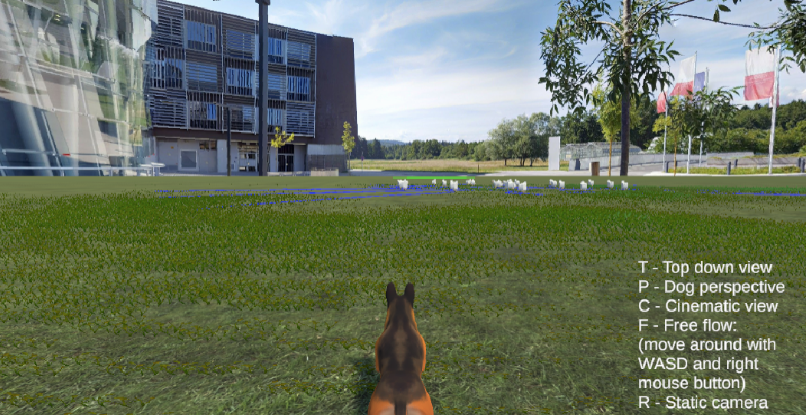
\includegraphics[width=\textwidth]{fig/dogp.PNG}
        \caption{Caption for Image 1}
    \end{subfigure}
    \hfill
    \begin{subfigure}{0.48\textwidth}
        \centering
        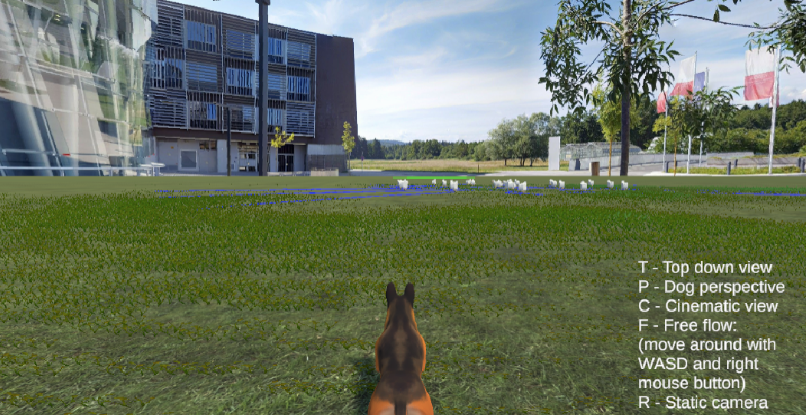
\includegraphics[width=\textwidth]{fig/dogp.PNG}
        \caption{Caption for Image 2}
    \end{subfigure}
    \\[1em] % Add space between rows
    \begin{subfigure}{0.48\textwidth}
        \centering
        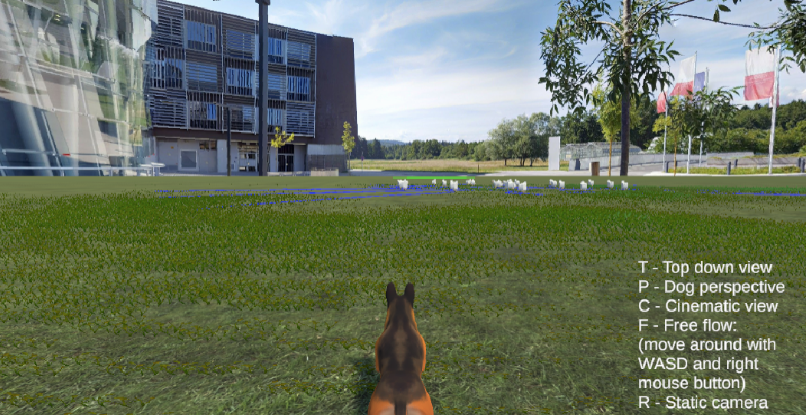
\includegraphics[width=\textwidth]{fig/dogp.PNG}
        \caption{Caption for Image 3}
    \end{subfigure}
    \hfill
    \begin{subfigure}{0.48\textwidth}
        \centering
        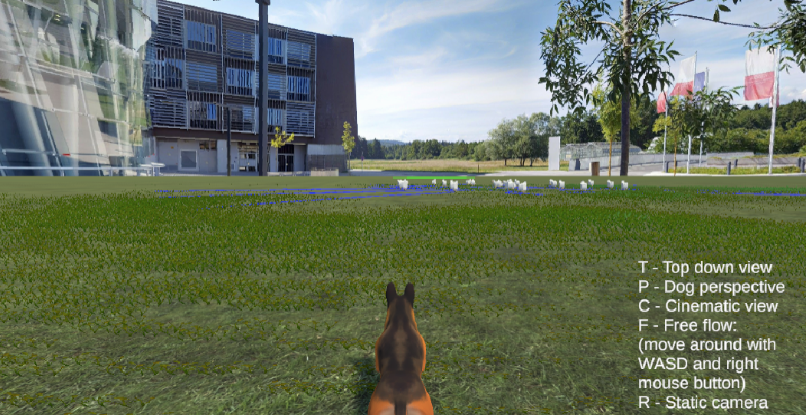
\includegraphics[width=\textwidth]{fig/dogp.PNG}
        \caption{Caption for Image 4}
    \end{subfigure}
    \\[1em] % Add space below the last row
    \begin{subfigure}{0.48\textwidth}
        \centering
        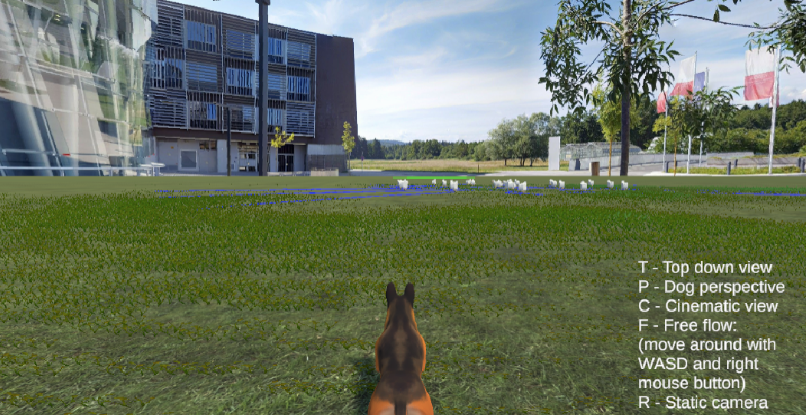
\includegraphics[width=\textwidth]{fig/dogp.PNG}
        \caption{Caption for Image 5}
    \end{subfigure}
    \caption{Grid of Images showing different views or examples.}
    \label{fig:grid}
\end{figure}
\end{comment}

\begin{figure}[H]
	\centering
	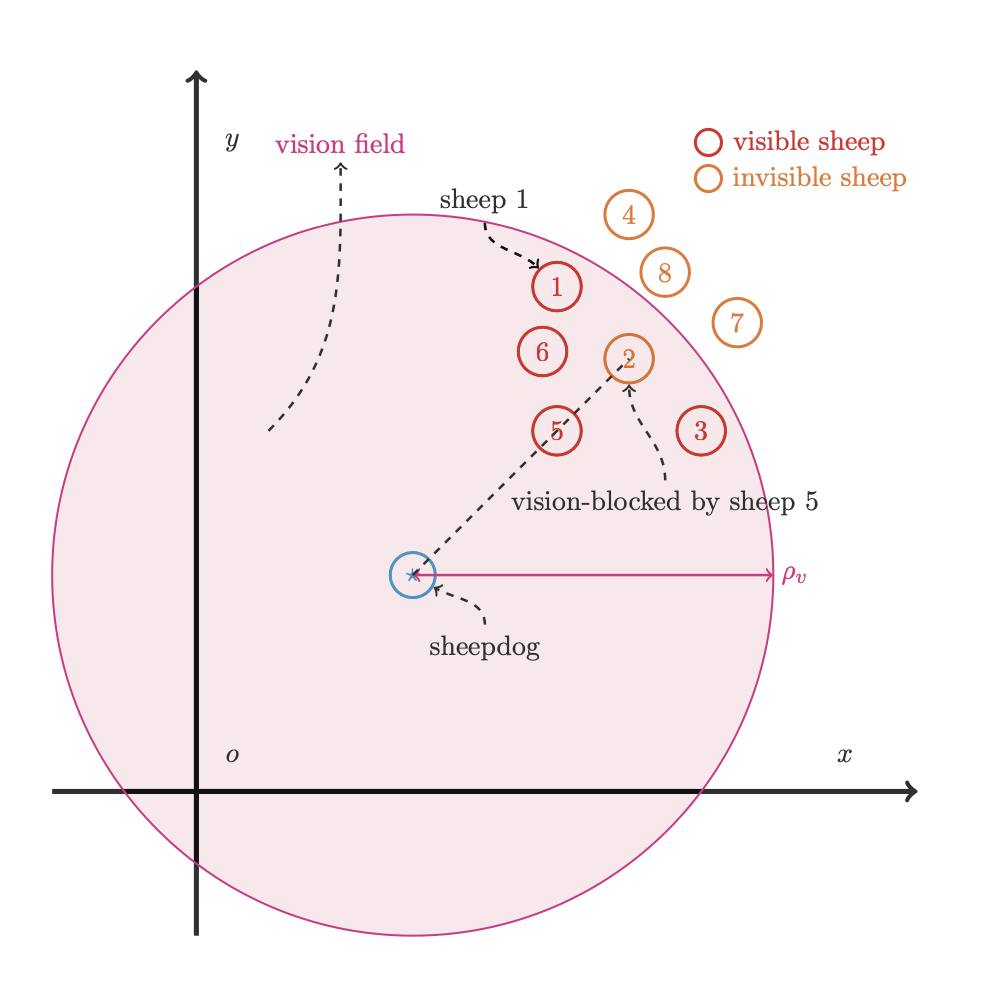
\includegraphics[width=.5\linewidth]{fig/vision-field.png}
	\caption{Example of dog's field of view.\cite{liu2021}}
	\label{fig:vision-field}
\end{figure}

The control process of the sheepdog is divided into two phases:
\begin{enumerate}
    \item Initialization: This phase involves setting key design parameters such as viewing angles, approach distances, and thresholds for direction adjustments. A time limit is also set for the operation.
    \item Iteration: In the main phase, the algorithm evaluates the position of the sheep relative to the target and adjusts the sheepdog's movement accordingly. The sheepdog decides whether to move directly toward the herd or to take a detour based on the herd's overall position. When detouring, it aligns itself with the rightmost or leftmost visible sheep, adjusting its angle to efficiently steer the herd without unnecessary deviation from the target path.
\end{enumerate}

The algorithm operates through a series of conditions to ensure energy efficiency and maintain herd cohesion, continuing until all sheep are guided to the target area or the time limit is reached.

%The algorithm itself serves as the foundation for the Simulation phase, where its implementation will be tested and refined in a Python-based environment. Following the algorithm's execution, its performance will be evaluated in simulated conditions, with particular attention to the adaptability and effectiveness of the sheepdog’s control in various test scenarios.

\subsection*{Object-Oriented Approach}
To simulate the behavior of the sheep and the dog, we employed an object-oriented programming approach
using Python.

The core of the simulation is encapsulated within the Simulation class.
All fixed parameters, such as the number of sheep, the destination position (sheepfold),
the attraction radius, and the safety radius, are defined as class variables.
Additionally, the current positions of the sheep and the dog are stored as NumPy arrays,
ensuring efficient computation and manipulation.

\subsection*{Simulation}

The simulation operates as a series of discrete steps. At the beginning of each step,
the algorithm checks if convergence has been achieved—specifically, whether all sheep are within
the destination circle. If this condition is met, the algorithm terminates. Otherwise,
the simulation proceeds to calculate the updated positions of the dog and sheep.

\begin{enumerate}
    \item Dog Movement:
    A velocity vector is computed for the dog. This velocity is scaled by a sampling period T and added to the previous position of the dog to determine its new position.
    \item Sheep Movement:
    Each sheep’s velocity is calculated based on its current state. This velocity is then transformed using a rotation matrix and added to its previous position.
\end{enumerate}

After updating the positions, the step counter is incremented, and the old positions are stored.
This historical data is essential for generating visualizations, as it provides the trajectory
of both the sheep and the dog.

A simple visualization was implemented during development as a Python scatter plot.
In this plot, the sheep and dog are represented by points of different colors,
providing an intuitive view of their movements. 

\begin{figure}[H]
	\centering
	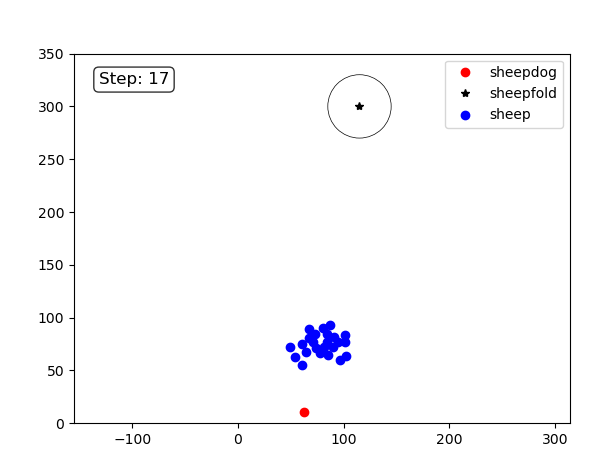
\includegraphics[width=.5\linewidth]{fig/step17.PNG}
	\caption{A simple visualization of the starting phase of herding.}
	\label{fig:start}
\end{figure}

\subsection*{Visualization} \label{vis}
The more polished and informative visualization component of the project was developed in Unity to render movement data generated from the Python simulation, offering an interactive and insightful format for analyzing the algorithm's behavior. The goal was to create an intuitive environment where the guiding of the herd by the sheepdog under various conditions could be observed.

Path data from the Python simulation was imported into Unity to initiate the visualization. This data, in the form of .json files, represented the movement of each entity (sheep and sheepdog) and enabled the creation of animated paths that reflected their interactions over time. A virtual environment was constructed in Unity to visually simulate the conditions modeled in Python.

The scene was managed by a core object called the "Manager", which dynamically generated all entities based on the .json data. This included determining the number of sheep, dogs, their starting positions, and the destination points. Parameters such as simulation speed and the visualization of entity paths were able to be adjusted during runtime. A graphical representation of the dog and sheep was included, with the option to replace these models.

A flat terrain with textures and painting details was created using Unity’s tools to ensure a realistic environment. A skybox featuring a 360° photo of the FRI campus in Ljubljana was included, setting the stage for a more realistic and interesting simulation.

Multiple techniques were employed to highlight critical aspects of the algorithm. Path trails, speed indicators, and field-of-view displays were used to emphasize the dynamics between the sheepdog and the herd. The LineRenderer, assigned by the Manager, rendered each entity’s path. As the simulation progressed, entities moved at the same speed from one coordinate to the next, with smooth transitions between points. The rotation of each entity was updated so that they faced the direction in which they moved, using linear interpolation for smooth transitions.

In addition to the core functionality, five different camera modes were implemented, with smooth transitions between them. These modes allow the user to switch between perspectives such as the dog’s point of view and a top-down view of the simulation.



\begin{figure}[htbp]
    \centering
    \begin{minipage}{0.3\textwidth}
        \centering
        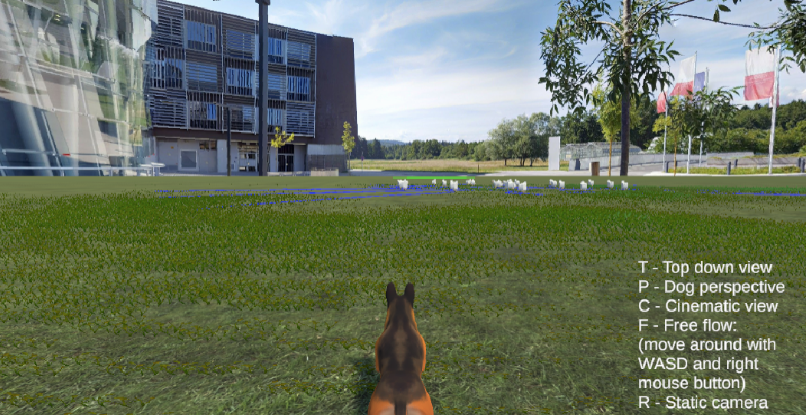
\includegraphics[width=\textwidth]{fig/dogp.PNG}
        \caption{Example of a dog perspective view.}
    \end{minipage}%
    \hspace{0.02\textwidth}  % Horizontal space between images
    \begin{minipage}{0.3\textwidth}
        \centering
        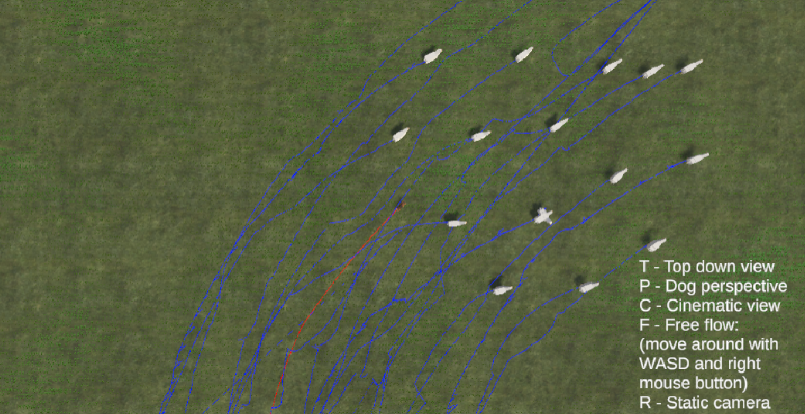
\includegraphics[width=\textwidth]{fig/topdown.PNG}
        \caption{Example of a top down view.}
    \end{minipage}%
    \hspace{0.02\textwidth}  % Horizontal space between images
    \begin{minipage}{0.3\textwidth}
        \centering
        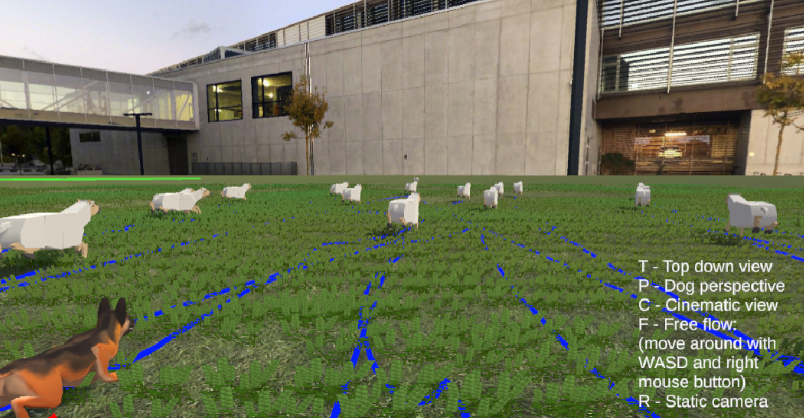
\includegraphics[width=\textwidth]{fig/cinematic.PNG}
        \caption{Example of a cinematic view.}
    \end{minipage}
    
    \vspace{0.4cm}  % Vertical space between the rows

    \begin{minipage}{0.3\textwidth}
        \centering
        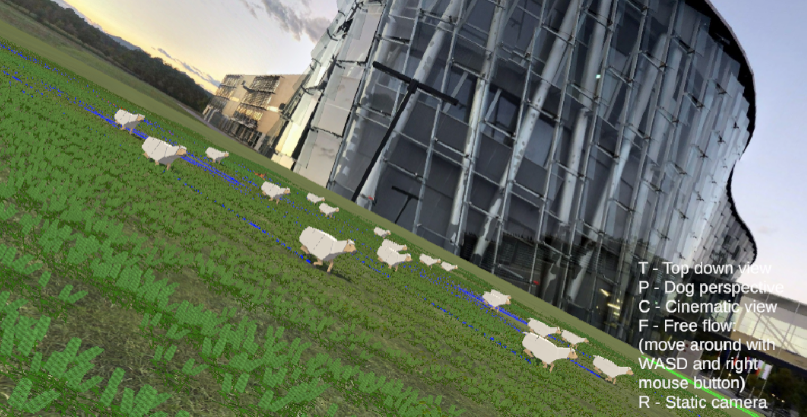
\includegraphics[width=\textwidth]{fig/freeflow.PNG}
        \caption{Example of a free flow view.}
    \end{minipage}%
    \hspace{0.02\textwidth}  % Horizontal space between images
    \begin{minipage}{0.3\textwidth}
        \centering
        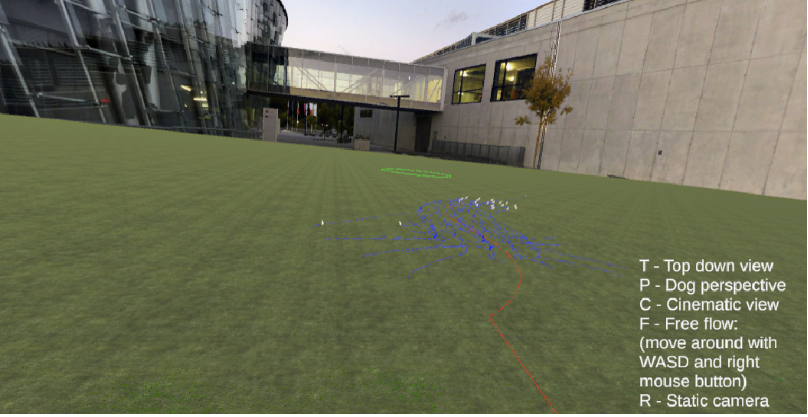
\includegraphics[width=\textwidth]{fig/static.PNG}
        \caption{Example of a static camera view.}
    \end{minipage}
\end{figure}

During the development of the simulation, challenges emerged in ensuring smooth transitions between coordinates and preventing overflows. These challenges were resolved through custom code, which provided full control over the entities’ movement and positioning.


\section*{Results}

The Sheepdog-Driven Algorithm for Sheep Herd Transport was  implemented, recreating the core framework described in the original paper. The interactions between the sheepdog and the sheep were modeled using local interaction rules, with the dog designed to guide the herd toward a target destination. Movement dynamics, including attraction, repulsion, and visibility checks, were incorporated, and the agents' positions were updated in real-time to simulate natural behavior.

A 3D visualization was developed to illustrate the algorithm’s dynamics, providing an intuitive representation of the interactions between the sheepdog and the herd. The visualization allowed for a detailed analysis of movement patterns and the algorithm’s performance under varying conditions.

However, despite closely following the methodology, the simulation did not consistently achieve the intended outcome of guiding the herd to the designated target. While the sheep’s movements responded to the sheepdog as expected, the dog was unable to reliably lead the herd to the goal. These results suggest potential areas for refinement in the algorithm’s implementation, which are discussed further in the next section.





\section*{Discussion}

The implementation of the \textit{Sheepdog-Driven Algorithm} revealed several challenges that impacted the consistency of the results. A primary issue was the lack of clarity and detail in the original paper, which introduced numerous terms and variables without sufficient definitions or context.

To give a few examples, the terms \(S_r(p_d - x)\) and \(S_l(p_d - x)\), introduced in \cite{liu2021}, were not explained in terms of their practical computation. Similarly, the variable \(D_q^d(k)\), intended to represent the direction from the sheepdog to the sheepfold, was not used in subsequent equations or pseudocode, adding to the ambiguity.

While some terms, such as \(o(x) = \frac{x}{|x|}\), were defined mathematically, their interactions with other variables, like \(p_q^i(k)\) and \(p_d^i(k)\), were not fully clarified. Additionally, the "sheep herd polygon" function \(P_s(k)\) was introduced but not explicitly utilized, leaving its purpose unclear.

After following the algorithm as described, unexpected behavior was observed, with the sheepdog initially moving away from the sheep rather than guiding them. A correction was made by reversing the sign in the \(o(q(k) - D_l(k))\) function, which resolved the issue and allowed the sheepdog to interact with the herd more effectively. However, no justification for this adjustment was provided in the paper, and it remains unclear if this modification aligns with the intended algorithm design.

The authors were contacted for clarification, but no response was received. This lack of guidance required reliance on trial and error, independent research, and assumptions to address the gaps in the paper. While this approach allowed for partial implementation of the algorithm, some ambiguities remained unresolved. Moreover, the paper itself is not so well-suited for direct implementation, and there is no open-source implementation available.

Despite these challenges, the visualization highlighted the effectiveness of certain behaviors, such as the sheep responding to the sheepdog’s position. However, the inability to consistently guide the herd to the target suggests areas for further refinement, including adjustments to the dog’s guidance strategy and cohesion dynamics within the herd.




\subsection*{Contributions}
IB and SH did the implementation, LP did visualizations, II did the report.

\begin{multicols}{2}
\section*{\bibname}
% Bibliography
\bibliography{./bib/bibliography}
\end{multicols}

\end{document}
